\documentclass[sigconf]{acmart}

\title{Modular and Multithreaded Web Crawler for Corpus Collection}


\author{Gabriel Teixeira Carvalho}
\affiliation{%
  \institution{Universidade Federal de Minas Gerais}
  \city{Belo Horizonte}
  \state{MG}
  \country{Brazil}
}
\email{gteixeiraca@gmail.com}
\settopmatter{printacmref=false}
\setcopyright{none}
\renewcommand\footnotetextcopyrightpermission[1]{}
\pagestyle{plain}
\begin{document}

\begin{abstract} 
This report presents the development of a modular and multithreaded web crawler designed to efficiently fetch a corpus of webpages while respecting politeness policies. The system integrates URL frontier management, HTML parsing, compliant page fetching, and WARC file storage. Through multithreading, the crawler achieved an average rate of 6.64 pages per second across 100,000 pages from 1,319 unique domains. We discuss the computational complexity of key modules, analyze empirical performance including download rates and speedups with varying thread counts, and provide a statistical characterization of the collected corpus.
\end{abstract}

\keywords{Information Retrieval, Web Crawling, Multithreading, Corpus Collection}

\maketitle
\acmConference{Information Retrieval}{April 2025}{Belo Horizonte, MG, Brazil}

\section{Introduction}
Web crawlers are fundamental tools for collecting large-scale datasets for research and applications in information retrieval. This work describes the design and implementation of a multithreaded web crawler capable of efficiently gathering a mid-sized corpus while adhering to site-specific access policies defined in robots.txt files. The crawler was structured into modular components focusing on URL management, fetching, parsing, storage, and logging, with multithreading enhancing throughput. Throughout the project, we evaluated computational complexities and measured empirical performance, providing insights into the crawler's scalability and efficiency across different thread counts.


\section{Data Structures and Algorithm}
\subsection{Crawler}
The \texttt{Crawler} class coordinates the overall crawling process by managing multiple worker threads. Each worker repeatedly fetches, parses, stores, and logs webpages while respecting a global crawling limit.

Upon initialization, the crawler sets up essential components: \texttt{Frontier} for URL management, \texttt{Fetcher} for downloading pages with politeness, \texttt{Parser} for HTML content extraction, \texttt{Storer} for WARC file writing, and \texttt{Logger} for debug logging. A global thread-safe counter tracks the remaining number of pages to fetch.

Each thread executes a method that performs the following steps:
\begin{itemize}
  \item Fetches the next URL from the \texttt{Frontier}.
  \item Requests the page content using \texttt{Fetcher}.
  \item Parses the HTML to extract links and metadata with \texttt{Parser}.
  \item Stores the fetched content using \texttt{Storer} and logs metadata via \texttt{Logger}.
  \item Adds newly discovered URLs to the \texttt{Frontier}.
\end{itemize}

Synchronization across threads is achieved using a \texttt{Lock} to protect updates to the crawling limit and a \texttt{stop\_signal} event to safely terminate threads when the crawling goal is reached or no URLs remain. Exception handling ensures that unexpected errors are logged and do not crash the entire crawler.

Overall, the crawler's architecture enables high concurrency, robustness, and modularity, facilitating efficient web-scale data collection.

\subsection{Frontier}
The \texttt{Frontier} class manages the set of URLs to be crawled using a thread-safe queue. It ensures that each URL is visited at most once by maintaining a \texttt{visited} set. The frontier supports basic operations like retrieving the next URL and adding new URLs. URLs are normalized to avoid duplicates caused by superficial formatting differences. A maximum crawling depth can be enforced, and a timeout mechanism ensures that crawler threads do not block indefinitely when the queue is empty. The frontier only accepts HTTP and HTTPS URLs.

\subsection{Fetcher}
The \texttt{Fetcher} class is responsible for downloading webpages while adhering to the crawling policies defined in each site's \texttt{robots.txt} file. It maintains a dictionary that maps domains to parsed \texttt{robots.txt} rules using the Protego library to avoid repeated downloads and policy parsing for the same domain.

Before fetching a URL, the \texttt{Fetcher} verifies access permission through the cached robots policy and applies a crawl delay, either specified by the website or a default setting. Fetch operations are executed via a persistent HTTP session, improving efficiency by reusing TCP connections.

The fetcher enforces both connection and read timeouts to prevent stalled requests from blocking threads indefinitely. Only content explicitly marked as \texttt{text/html} is retained; non-HTML content is ignored. Fault tolerance is incorporated: if a fetch operation fails due to invalid URLs, connection errors, or disallowed accesses, it returns safely without crashing the thread.

\subsection{Parser}
The \texttt{Parser} class extracts links and the HTML content from the fetched pages. It uses the BeautifulSoup library to parse the HTML and extract the relevant data. The links are added to the \texttt{Frontier} for further crawling, while the HTML content is passed to the \texttt{Storer} for storage. Additionally, it extracts the page title and the first 20 words of the body text for logging purposes.

\subsection{Storer}
The \texttt{Storer} class is responsible for writing the fetched pages to WARC files. It uses the warcio library to create and manage WARC files, ensuring that each page is stored with its metadata. The storer handles file rotation when a certain size limit is reached, creating new WARC files as needed, with a default size of 1000 pages per file. The storer uses a lock to ensure that multiple threads do not write to the same file simultaneously, preventing data corruption.

\subsection{Logger}
The \texttt{Logger} class is responsible for logging the crawling process. If debugging is enabled, each thread calls the \texttt{Logger} to log the URL being fetched, the title of the page, the text content, and the timestamp of the fetch operation. The logger uses a dedicated thread to write logs to a file, ensuring that logging does not block the main crawling threads. The log entries are saved in jsonl format, allowing for easy parsing and analysis later.


\section{Computational Complexity}
The computational complexity of the \texttt{Crawler} can be analyzed based on its main components:
\begin{itemize}
  \item \textbf{\texttt{Frontier}}: The complexity of adding and retrieving URLs is \texttt{O(1)} due to the use of a hash set for visited URLs and a queue for the frontier.
  \item \textbf{\texttt{Fetcher}}: The complexity of fetching a page is \texttt{O(p)}, where \texttt{p} is the size of the page. The time taken to parse the \texttt{robots.txt} file is negligible compared to the fetch time. Network latency and server response times are not included in this analysis, as they are highly variable.
  \item \textbf{\texttt{Parser}}: The complexity of parsing a page is \texttt{O(p)}, where \texttt{p} is the size of the page. The time taken to extract links and metadata is linear with respect to the size of the page.
  \item \textbf{\texttt{Storer}}: The complexity of writing to a \texttt{WARC} file is \texttt{O(p)}, where \texttt{p} is the size of the page. File rotation adds a constant overhead.
  \item \textbf{\texttt{Logger}}: The complexity of logging is \texttt{O(1)} for each log entry. However, when the \texttt{Logger} thread is writing to the log file, it may write up to \texttt{O(k)} entries at once, where \texttt{k} is the number of log entries accumulated since the last write. 
\end{itemize}

The overall complexity of the \texttt{Crawler} can be approximated as \texttt{O(p * n)}, where \texttt{p} is the average size of the pages and \texttt{n} is the number of pages crawled. The multithreading aspect allows for concurrent execution, which can significantly reduce the effective time taken to crawl a large number of pages. The actual performance gain depends on the number of threads and the network conditions, with network latency and server response times being the main bottlenecks. 

\section{Results}
\subsection{Crawling Performance}
The crawler was run with different thread counts to evaluate its performance using a limit of 2,000 pages. The following table summarizes the results:
\begin{table}[H]
\centering
\begin{tabular}{|c|c|}
\hline
\textbf{Threads} & \textbf{Download rate (pages / sec)} \\ \hline
1 & 0.8745 \\ \hline
10 & 6.6085 \\ \hline
25 & 5.6072 \\ \hline
50 & 7.4239 \\ \hline
100 & 7.5306 \\ \hline
200 & 7.3023 \\ \hline
500 & 7.2017 \\ \hline
\end{tabular}
\caption{Crawling performance with different thread counts}
\label{tab:performance}
\end{table}
The table shows the number of threads used and the corresponding download rate in pages per second. The results indicate that increasing the number of threads significantly improves the download rate, with a peak at 100 threads.
However, the performance starts to decrease beyond this point, suggesting that the network bandwidth, server response times and timeouts may become limiting factors.

\subsection{Corpus Characterization}
After we defined the best thread count, we crawled a total of 100,000 pages starting with the following seed URLs:
\begin{itemize}
  \item \url{http://www.band.com.br/}
  \item \url{http://news.google.com.br/}
  \item \url{https://www.bol.uol.com.br/}
\end{itemize}

The following table summarizes the corpus characteristics:
\begin{table}[H]
\centering
\begin{tabular}{|c|c|}
\hline
\textbf{Metric} & \textbf{Value} \\ \hline
Number of pages & 100,000 \\ \hline
Number of unique domains & 1,319 \\ \hline
Average number of pages per domain & 75.8862 pages\\ \hline
Average download rate & 6.64 pages/sec\\ \hline
Average page size & 243521.24 bytes \\ \hline
Average tokens per page & 3082.45 tokens \\ \hline
Average out-links per page: &  360.31 links \\ \hline
\end{tabular}
\caption{Corpus characteristics}
\label{tab:corpus}
\end{table}
The results indicate that the crawler was able to collect a large and diverse corpus of webpages.

\subsection{Distribution of Pages per Domain}
The following histogram shows the distribution of pages per domain in the corpus:
\begin{figure}[h]
\centering
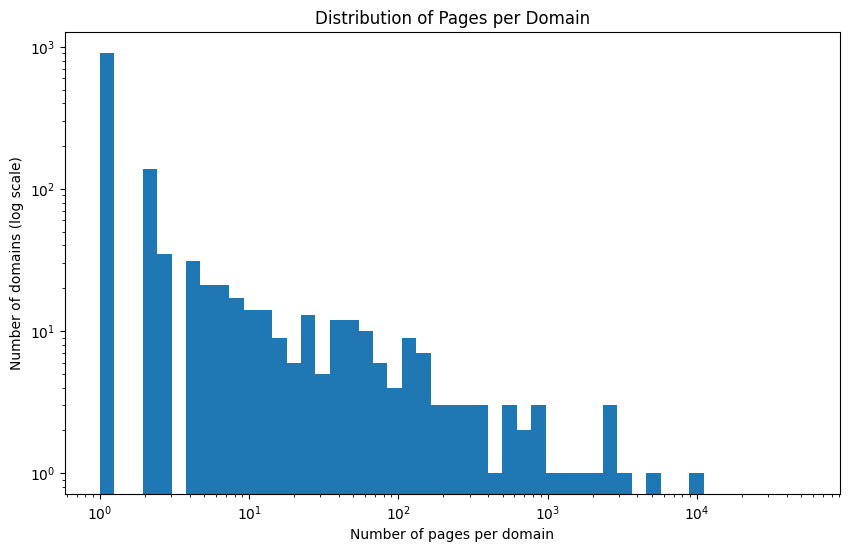
\includegraphics[width=0.8\linewidth]{acmart-primary/acmart-primary/samples/pages_per_domain.png}
\caption{Distribution of pages per domain}
\label{fig:histogram}
\end{figure}
The histogram shows that most domains have a small number of pages, while a few domains have a large number of pages. This is expected, as some of the seed URLs are popular news sites that have a large number of pages under their domain. The average number of pages per domain is 75.8862 pages.

\subsection{Distribution of Tokens per Page}
The following histogram shows the distribution of tokens per page in the corpus:
\begin{figure}[H]
\centering
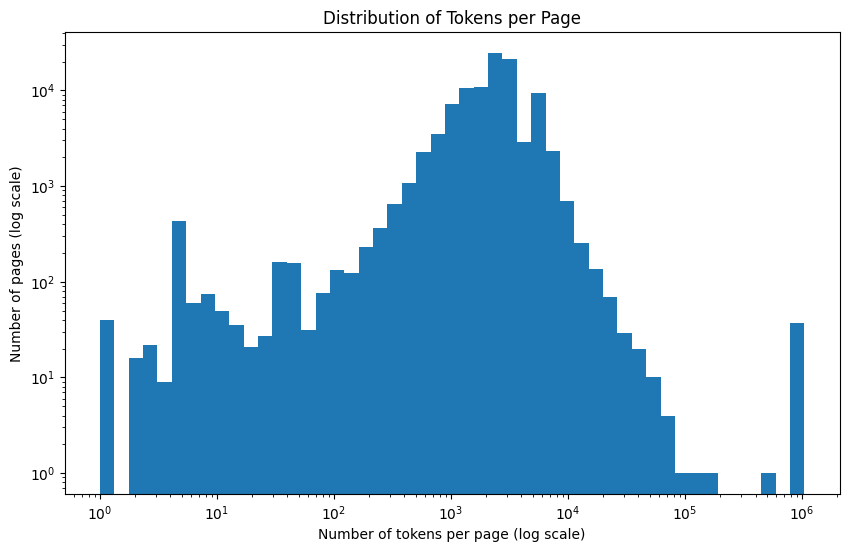
\includegraphics[width=0.8\linewidth]{acmart-primary/acmart-primary/samples/tokens_per_page.png}
\caption{Distribution of tokens per page}
\label{fig:histogram_tokens}
\end{figure}
The histogram shows that most pages have between 100 and 10,000 tokens, with some exceptions having more than 1,000,000 tokens. This is expected, as some pages are designed to be very long, such as articles or blog posts. The average number of tokens per page is 3,082.45.

\subsection{Distribution of Out-links per Page}
The following histogram shows the distribution of out-links per page in the corpus:
\begin{figure}[H]
\centering
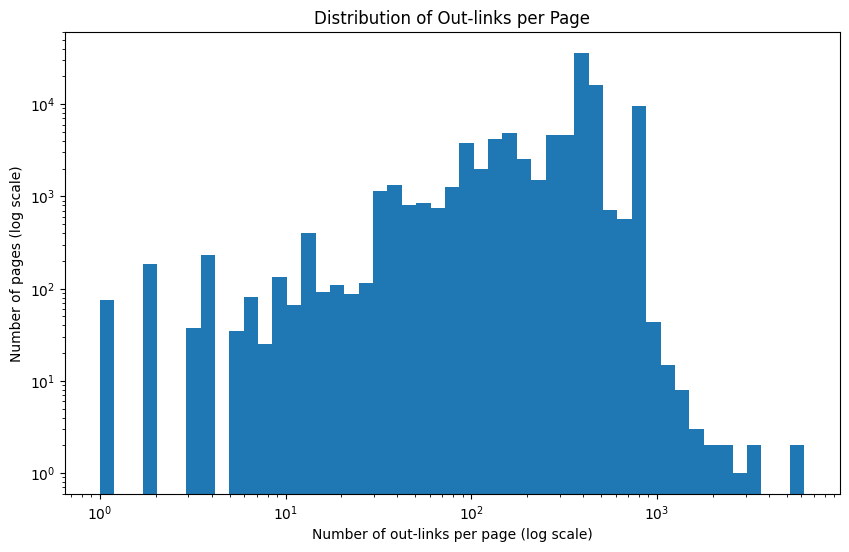
\includegraphics[width=0.8\linewidth]{acmart-primary/acmart-primary/samples/out_links_per_page.png}
\caption{Distribution of out-links per page}
\label{fig:histogram_links}
\end{figure}
The histogram shows that a lot of pages have between 100 and 1,000 out-links, while a few pages have a larger number of out-links. This is expected, as some pages are designed to link to many other pages, such as news aggregators or social media sites. The average number of out-links per page is 360.31 links.

\subsection{Most Frequent Domains}
The following table shows the most frequent domains in the corpus:
\begin{table}[H]
\centering
\begin{tabular}{|c|c|}
\hline
\textbf{Domain} & \textbf{Count} \\ \hline
www1.folha.uol.com.br & 52,497 \\ \hline
www.uol.com.br & 9,030 \\ \hline
brasilescola.uol.com.br & 5,283 \\ \hline
exercicios.brasilescola.uol.com.br & 2,960 \\ \hline
mundoeducacao.uol.com.br & 2,544 \\ \hline
escolakids.uol.com.br & 2,497 \\ \hline
f5.folha.uol.com.br & 2,460 \\ \hline
vestibular.brasilescola.uol.com.br & 1,931 \\ \hline
exercicios.mundoeducacao.uol.com.br & 1,723 \\ \hline
economia.uol.com.br & 1,367 \\ \hline
\end{tabular}
\caption{Most frequent domains in the corpus}
\label{tab:domains}
\end{table}

The table shows the most frequent domains in the corpus and the number of pages crawled from each domain. The results indicate that the crawler was able to collect a large number of pages from popular domains, which all belonged to UOL, a Brazilian news and content aggregator site. Since the crawler started with UOL as a seed URL, it is expected that the crawler would collect a large number of pages from this domain.

\section{Conclusion}
This report presents the design and implementation of a multithreaded web crawler capable of efficiently collecting a corpus of webpages while respecting site-specific access policies. The crawler's modular architecture allows for easy maintenance and scalability, while multithreading significantly enhances performance. Empirical results demonstrate the crawler's ability to achieve high download rates and collect a diverse set of webpages. The statistical characterization of the corpus provides insights into the distribution of pages, tokens, and out-links, highlighting the crawler's effectiveness in gathering web data, which is crucial for various applications in information retrieval.

\end{document}
